\documentclass[12pt,a4paper]{article}
\usepackage[utf8]{inputenc}
\usepackage[spanish,es-tabla]{babel}
\usepackage{geometry}
\usepackage{graphicx}
\usepackage{multirow}
\usepackage{tabularx}
\usepackage{mathptmx}
\usepackage{fancyhdr}
\usepackage{array}
\usepackage[table]{xcolor}
\usepackage{titlesec}
\usepackage{setspace}
\usepackage{microtype}
\usepackage{lastpage}
\usepackage{booktabs}
\usepackage{enumitem}
\usepackage{amsmath}
\usepackage{amsfonts}
\usepackage{amssymb}

\graphicspath{{images/}{../images/}{./}}

\geometry{
    top=4.7cm,
    bottom=2.5cm,
    left=2.5cm,
    right=2.5cm,
    headheight=3.9cm,
    headsep=0.4cm
}

\setstretch{1.15}
\setlength{\parindent}{0pt}
\setlength{\parskip}{0.45em}
\setlength{\tabcolsep}{4pt}

\titleformat{\section}
  {\normalfont\fontsize{12}{14.5}\bfseries}{\thesection.}{0.6em}{\uppercase}
\titlespacing*{\section}
  {0pt}{1.8ex plus 0.4ex minus 0.2ex}{0.6ex plus 0.2ex}

\titleformat{\subsection}
  {\normalfont\fontsize{11.5}{13.5}\bfseries}{\thesubsection.}{0.5em}{}
\titlespacing*{\subsection}
  {0pt}{1.4ex plus 0.3ex minus 0.1ex}{0.4ex plus 0.1ex}

\titleformat{\subsubsection}
  {\normalfont\fontsize{10.5}{12.5}\bfseries\itshape}{\thesubsubsection.}{0.4em}{}
\titlespacing*{\subsubsection}
  {0pt}{1.1ex plus 0.2ex minus 0.1ex}{0.3ex plus 0.1ex}

\newcolumntype{Y}{>{\centering\arraybackslash}X}
\newcolumntype{L}{>{\raggedright\arraybackslash}X}
\newcolumntype{C}{>{\centering\arraybackslash}X}

\definecolor{headerblue}{RGB}{26, 54, 93}
\definecolor{darkblue}{RGB}{43, 108, 176}
\definecolor{lightgraybg}{RGB}{248, 248, 248}
\definecolor{tableheader}{RGB}{232, 238, 246}

\newcommand{\docCodigo}{TI-SIGE-ENT-F2-007}
\newcommand{\docVersion}{1.0}
\newcommand{\docProceso}{HITO DE CONTROL / APROBACIÓN DE FASE 2}
\newcommand{\docElaboracion}{04/09/2026}
\newcommand{\docRevision}{04/09/2026}
\newcommand{\docTitulo}{HITO 2: APROBACIÓN DE ARQUITECTURA Y ENTREGABLE GENERAL}
\newcommand{\docOrganizacion}{FACULTAD DE INGENIERÍA EN SISTEMAS, ELECTRÓNICA E INDUSTRIAL}
\newcommand{\docSubOrganizacion}{CARRERA DE INGENIERÍA DE SOFTWARE}

\newcommand{\encabezadofrecuente}{%
    \renewcommand{\arraystretch}{1.15}%
    \noindent\makebox[\textwidth][c]{%
    \begin{tabularx}{\textwidth}{|>{\centering\arraybackslash}m{2.8cm}|Y|>{\centering\arraybackslash}m{4.8cm}|}
        \hline
        \multirow{4}{2.8cm}{\centering\raisebox{-1.15cm}{
\includegraphics[width=2.5cm,height=2.0cm,keepaspectratio]{images/logo.png}}}
        & \textbf{\fontsize{9}{11}\selectfont \docOrganizacion} 
        & \textbf{\fontsize{8}{10}\selectfont CÓDIGO:} \fontsize{8}{10}\selectfont \docCodigo \\
        \cline{3-3}
        & \textbf{\fontsize{8.5}{10.5}\selectfont \docSubOrganizacion} 
        & \textbf{\fontsize{8}{10}\selectfont VERSIÓN:} \fontsize{8}{10}\selectfont \docVersion \\
        \cline{2-3}
        & \textbf{\fontsize{8}{10}\selectfont PROCESO:} \fontsize{8}{10}\selectfont \docProceso 
        & \textbf{\fontsize{8}{10}\selectfont ELABORACIÓN:} \fontsize{8}{10}\selectfont \docElaboracion \\
        \cline{2-3}
        & \textbf{\fontsize{8.5}{10.5}\selectfont \docTitulo} 
        & \textbf{\fontsize{8}{10}\selectfont ÚLTIMA REVISIÓN:} \fontsize{8}{10}\selectfont \docRevision \\
        \hline
    \end{tabularx}%
    }%
}

\pagestyle{fancy}
\fancyhf{}
\fancyhead[C]{\encabezadofrecuente}
\fancyfoot[C]{\fontsize{10}{12}\selectfont Página \thepage\ de \pageref{LastPage}}
\renewcommand{\headrulewidth}{0pt}

\begin{document}

\noindent{\fontsize{10.5}{12.5}\selectfont \textbf{Integrantes:} Heidi Villavicencio \quad$\vert$\quad Steeven Toala \quad$\vert$\quad Nixon Hurtado \quad$\vert$\quad Andrea Vásquez}

\vspace{0.25cm}

\section{Título}
\textbf{Denominación del Entregable:} HITO 2: Aprobación de Arquitectura y Entregable General Semana 2 -- Código EDT: 2.7

\section{Introducción}
El cierre formal de la Fase 2: Diseño y Arquitectura representa el hito más crítico previo al inicio de la codificación y desarrollo del núcleo del sistema SIGE. En este documento se consolida la revisión exhaustiva de todos los artefactos de diseño construidos entre el 25 de agosto y el 04 de septiembre de 2026: Casos de Uso, Documento de Arquitectura de Software (SAD), Modelos Dinámicos UML, Base de Datos PostgreSQL 18, Wireframes y Prototipo Figma, y la Orquestación de Contenedores con Docker Compose. Se documenta la sustentación ante el docente evaluador Ing. Paulo Torres y la certificación formal para dar inicio al desarrollo Core en la Fase 3.

\section{Objetivo}
\subsection{Objetivo General}
Consolidar, evaluar y aprobar formalmente el paquete de entregables de la Fase 2: Diseño y Arquitectura (Hito 2), certificando la conformidad técnica y autorizando el inicio de la Fase 3 de Desarrollo Core.
\subsection{Objetivos Específicos}
\begin{itemize}[leftmargin=1.5em, itemsep=2pt]
    \item Verificar el cumplimiento y calidad técnica de los entregables EDT 2.1 al 2.6.
    \item Comprobar la trazabilidad del 100\% entre los Requerimientos SRS IEEE 830 y los artefactos de diseño arquitectónico.
    \item Realizar la demostración del prototipo interactivo en Figma y la puesta en marcha del stack Docker local.
    \item Suscribir el acta formal de aprobación de Hito 2 por parte del docente evaluador.
\end{itemize}

\section{Alcance}
\subsection{Límites del Entregable (In-Scope)}
\begin{itemize}[leftmargin=1.5em, itemsep=2pt]
    \item Consolidado de los 7 entregables de Fase 2 ejecutados entre el 25 de agosto y el 04 de septiembre de 2026.
    \item Validación de arquitectura de datos, interfaces y contenedores.
\end{itemize}
\subsection{Exclusiones (Out-of-Scope)}
\begin{itemize}[leftmargin=1.5em, itemsep=2pt]
    \item Cambios estructurales en el modelo relacional o arquitectura tras la firma de este hito.
\end{itemize}

\section{Definiciones}
\begin{itemize}[leftmargin=1.5em, itemsep=2pt]
    \item \textbf{Hito 2 (Milestone Semana 2):} Punto de control que certifica que los cimientos arquitectónicos del software están terminados y validados.
    \item \textbf{Línea Base de Arquitectura:} Conjunto congelado de especificaciones técnicas que guiarán la implementación del código fuente.
    \item \textbf{Trazabilidad Arquitectónica:} Capacidad de vincular cada requisito funcional con un componente o módulo específico del diseño.
\end{itemize}

\section{Responsabilidades}
\begin{itemize}[leftmargin=1.5em, itemsep=2pt]
    \item \textbf{Equipo de Proyecto SIGE (Responsables EDT 2.7):} Consolidación del paquete técnico, demostración de prototipos y sustentación.
    \item \textbf{Ing. Paulo Torres (Docente Evaluador / Patrocinador):} Revisión de conformidad, retroalimentación y suscripción formal de aprobación.
\end{itemize}

\section{Normativa Legal y Técnica}
\begin{itemize}[leftmargin=1.5em, itemsep=2pt]
    \item \textbf{IEEE Std 1016-2009:} Standard for Information Technology -- Systems Design -- Software Design Descriptions.
    \item \textbf{Guía PMBOK (7ma Edición):} Gestión de la Calidad y Cierre de Fase Técnica.
\end{itemize}

\section{Método, Políticas y Contenidos}
Se llevó a cabo una sesión de sustentación técnica de 2 horas el viernes 04 de septiembre de 2026. En la Figura \ref{fig:s2_07_cons} se presenta el mapa consolidado de la Fase 2 de Arquitectura.

\begin{figure}[htbp]
    \centering
    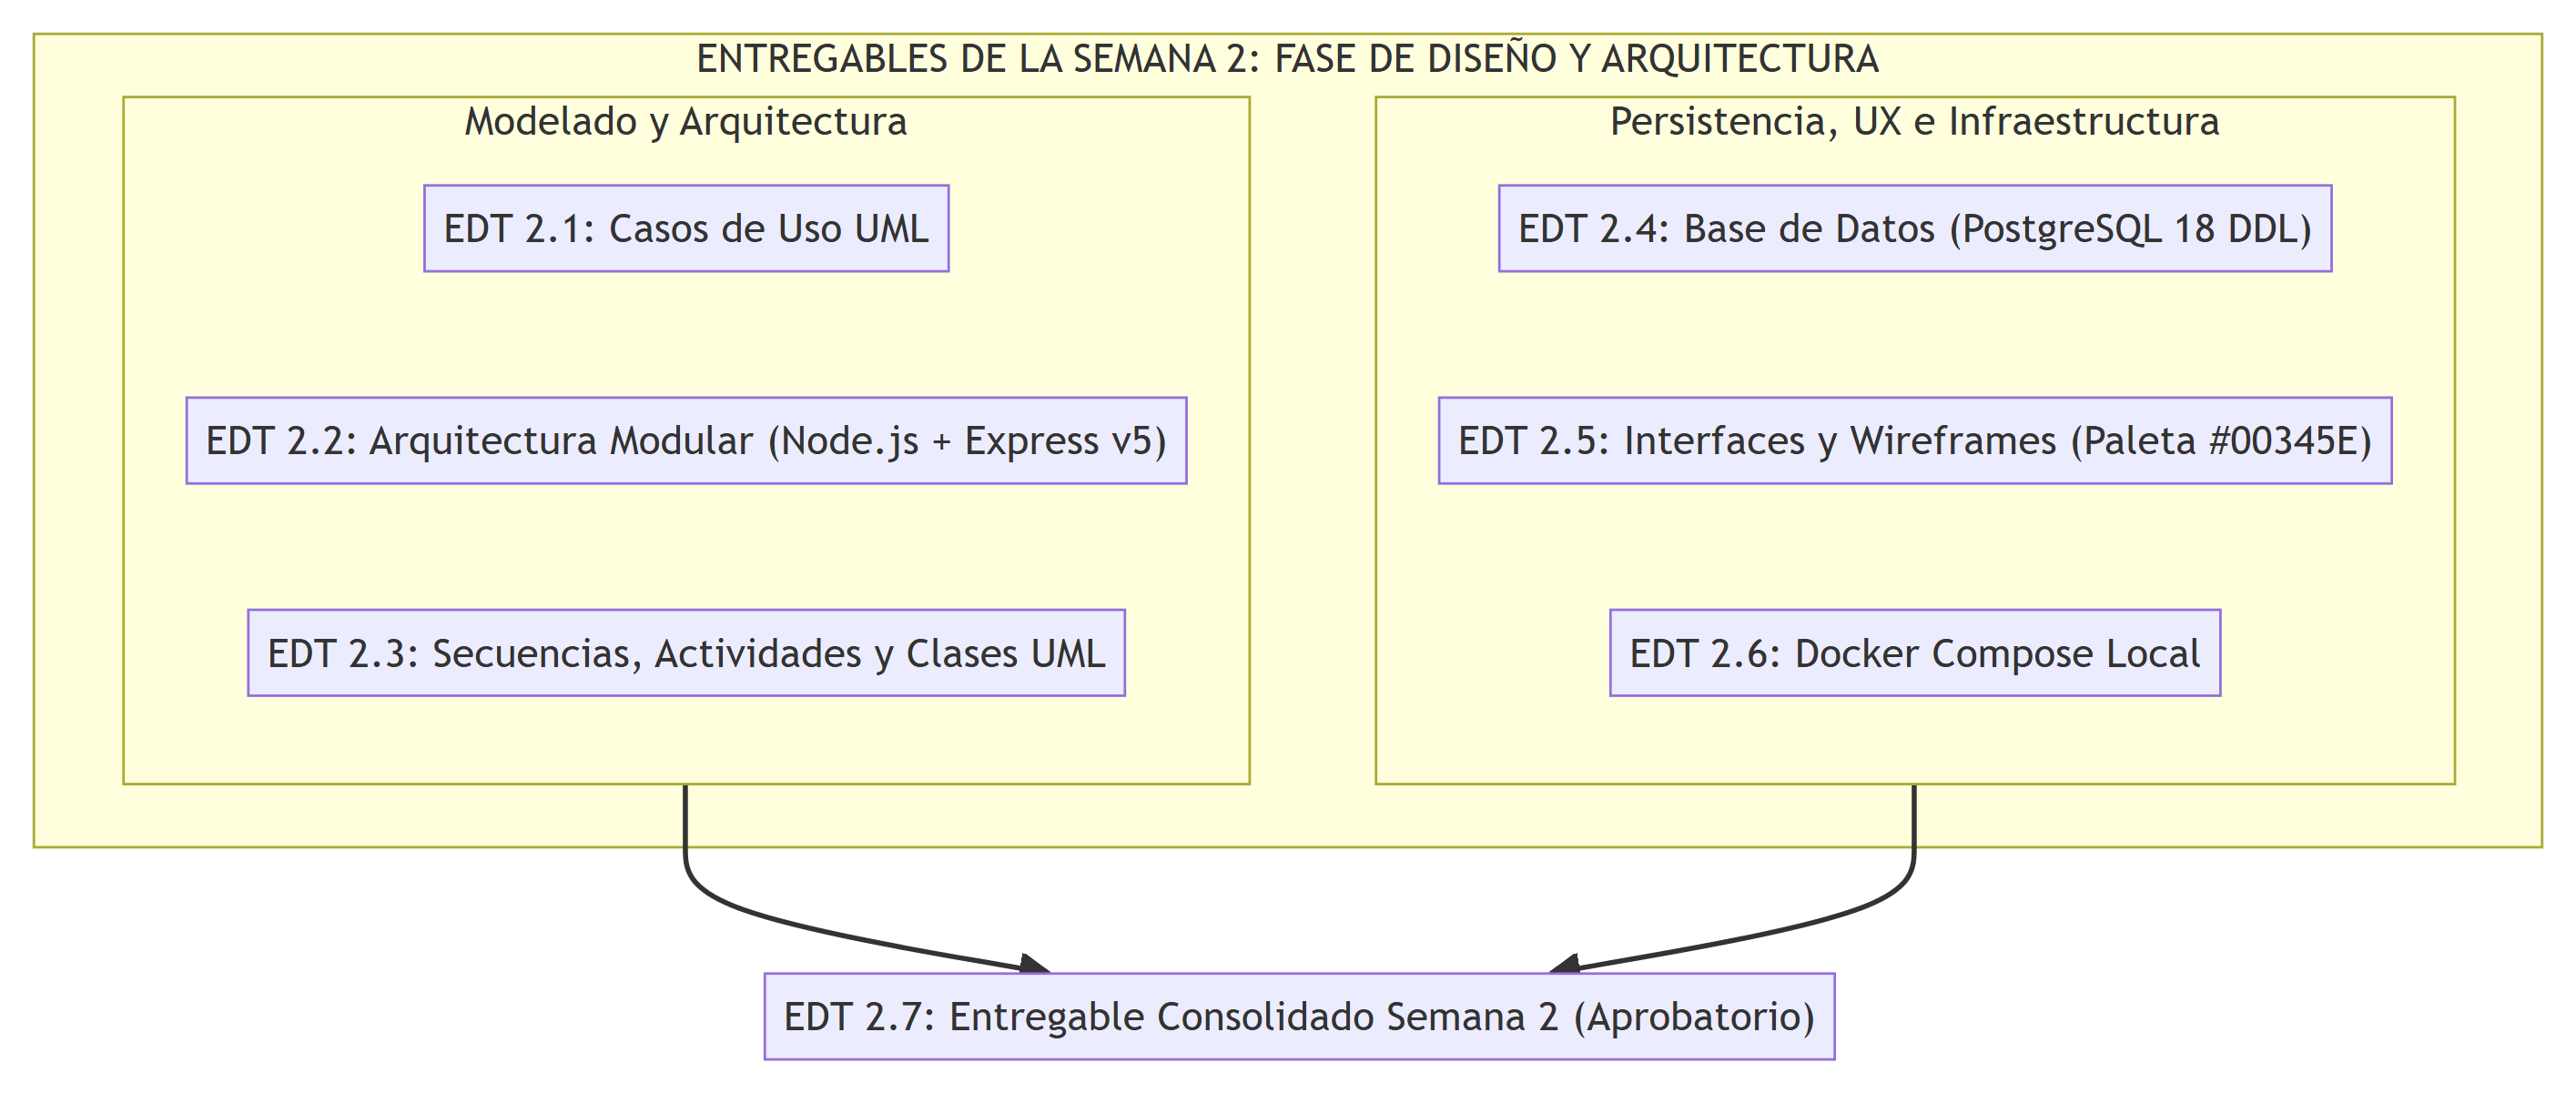
\includegraphics[width=0.85\textwidth,height=5.2cm,keepaspectratio]{images/s2_07_consolidado_s2.png}
    \caption{Mapa Consolidado de la Fase 2: Diseño y Arquitectura de la Solución.}
    \label{fig:s2_07_cons}
\end{figure}

\section{Descripción de actividades}
\subsection{Matriz de Verificación y Conformidad de Entregables de Fase 2}
\begin{table}[htbp]
\centering
\small
\renewcommand{\arraystretch}{1.2}
\begin{tabularx}{\textwidth}{|c|>{\bfseries}m{4.0cm}|X|c|c|}
\hline
\rowcolor{tableheader}
\textbf{EDT} & \\textbf{Entregable Oficial} & \textbf{Artefacto Verificado} & \textbf{Horas} & \textbf{Estado} \\
\hline
2.1 & Casos de Uso UML & Diagrama general y especificación CU-01 a CU-08 & 24 h & Aprobado \\
\hline
2.2 & Arquitectura SAD & Clean Architecture, C4 Model Nivel 1 y 2 & 32 h & Aprobado \\
\hline
2.3 & Modelado Dinámico & Diagramas Secuencia, Actividades y Clases & 40 h & Aprobado \\
\hline
2.4 & Base de Datos & ER Crow's Foot, normalización 3NF y 13 tablas & 40 h & Aprobado \\
\hline
2.5 & Interfaces y UX & Wireframes alta fidelidad, Wizard y Figma & 40 h & Aprobado \\
\hline
2.6 & Contenedores Docker & \texttt{docker-compose.yml}, PostgreSQL, MinIO, LT & 32 h & Aprobado \\
\hline
2.7 & Hito 2: Aprobación Arquitectura & Paquete Arquitectura Aprobado y Sustentación & 0 h & Aprobado \\
\hline
\multicolumn{3}{|r|}{\textbf{TOTAL HORAS INVERTIDAS EN FASE 2:}} & \textbf{208 h} & \textbf{100\%} \\
\hline
\end{tabularx}
\caption{Matriz de Conformidad y Cierre de Entregables de Fase 2.}
\label{tab:cierre_fase2}
\end{table}

\subsection{Dictamen Técnico y Autorización de Desarrollo}
El docente evaluador Ing. Paulo Torres emite el dictamen de APROBADO sin observaciones impeditivas, autorizando formalmente al equipo para iniciar la Fase 3: Desarrollo Core a partir del lunes 07 de septiembre de 2026.

\section{Firmas de Responsabilidad}

\noindent
\renewcommand{\arraystretch}{1.2}
\begin{tabularx}{\textwidth}{|>{\raggedright\arraybackslash}m{2.9cm}|>{\raggedright\arraybackslash}X|>{\centering\arraybackslash}m{4.6cm}|>{\centering\arraybackslash}m{2.3cm}|}
    \hline
    \rowcolor{tableheader}
    \textbf{ACCIÓN} & \textbf{NOMBRE Y CARGO} & \textbf{FIRMA} & \textbf{FECHA} \\
    \hline
    \textbf{Elaborado por:} & Heidi Villavicencio\newline Analista de Calidad / UI-UX & \parbox[c]{4.4cm}{\centering\vspace{4pt}
\includegraphics[height=1.5cm,width=4.0cm,keepaspectratio]{images/firma_heidi.png}\vspace{4pt}} & 04/09/2026 \\
    \hline
    \textbf{Revisado por:} & Steeven Toala\newline Líder de Proyecto / Arquitecto & \parbox[c]{4.4cm}{\centering\vspace{4pt}
\includegraphics[height=1.5cm,width=4.0cm,keepaspectratio]{images/firma_steveen.png}\vspace{4pt}} & 04/09/2026 \\
    \hline
    \textbf{Aprobado por:} & Ing. Paulo Torres, Mg.\newline Docente Evaluador -- Gestión Proyectos & \parbox[c]{4.4cm}{\centering\vspace{8pt}\textbf{\textcolor{gray!80}{\scriptsize [ PENDIENTE DE APROBACIÓN ]}}\vspace{8pt}} & \textbf{\textcolor{gray!90}{Pendiente}} \\
    \hline
\end{tabularx}

\vspace{0.4cm}

\section{Control de Cambios}

\noindent
\renewcommand{\arraystretch}{1.2}
\begin{tabularx}{\textwidth}{|>{\hsize=0.45\hsize\centering\arraybackslash}X|>{\hsize=1.55\hsize\raggedright\arraybackslash}X|>{\hsize=1.2\hsize\raggedright\arraybackslash}X|>{\hsize=0.8\hsize\centering\arraybackslash}X|}
    \hline
    \rowcolor{tableheader}
    \textbf{Versión} & \textbf{Descripción del cambio} & \textbf{Responsable del cambio} & \textbf{Fecha de aprobación} \\
    \hline
    1.0 & Emisión inicial del entregable según EDT del Tablero Trello & Equipo de Proyecto SIGE & 04/09/2026 \\
    \hline
\end{tabularx}

\vspace{0.4cm}

\section{Anexos}
\begin{itemize}[leftmargin=1.5em]
\item \textbf{Anexo 1:} Acta de Aprobación de Hito 2 (Semana 2).
\item \textbf{Anexo 2:} Matriz de Trazabilidad Arquitectura vs. Requerimientos SRS.
\end{itemize}

\end{document}
